\documentclass[12pt]{article}
\usepackage{hyperref}
\usepackage{listings}
\usepackage[margin=1in]{geometry}
\usepackage{enumitem}
\usepackage{multicol}
\usepackage{array}
\usepackage{titlesec}
\usepackage{helvet}
\renewcommand{\familydefault}{\sfdefault}
\usepackage{amsmath}     % For math equations
\usepackage{amssymb}     % For advanced math symbols
\usepackage{amsfonts} % For math fonts
\usepackage{gvv}
\usepackage{esint}
\usepackage[utf8]{inputenc}
\usepackage{graphicx}
\usepackage{pgfplots}
\pgfplotsset{compat=1.18}
\titleformat{\section}{\bfseries\large}{\thesection.}{1em}{}
\setlength{\parindent}{0pt}
\setlength{\parskip}{6pt}
\usepackage{multirow}
\usepackage{float}
\usepackage{caption}


\begin{document}

\textbf{Problem 7.3.5}

If a circle passes through the points $(0,0)$, $(a,0)$ and $(0,b)$, then find the coordinates of its centre.

\textbf{Input Variables}

\begin{table}[H]
\centering
\begin{tabular}{|c|c|}
\hline
Variable & Description \\
\hline
$\vec{x}_1 = \myvec{0 \\ 0}$ & First point on circle \\
\hline
$\vec{x}_2 = \myvec{a \\ 0}$ & Second point on circle \\
\hline
$\vec{x}_3 = \myvec{0 \\ b}$ & Third point on circle \\
\hline
\end{tabular}
\end{table}

\textbf{Solution}

From (7.1.3.1), for three points $\vec{x}_1, \vec{x}_2, \vec{x}_3$ on a circle:
\begin{align}
\myvec{
2\vec{x}_1 & 2\vec{x}_2 & 2\vec{x}_3 \\
1 & 1 & 1
}^\top
\myvec{\vec{u} \\ f}
=
-\myvec{\|\vec{x}_1\|^2 \\ \|\vec{x}_2\|^2 \\ \|\vec{x}_3\|^2},
\quad
\vec{c} = -\vec{u}.
\end{align}

Substituting the given points:
\begin{align}
\myvec{
0 & 2a & 0 \\
0 & 0 & 2b \\
1 & 1 & 1
}^\top
\myvec{u_1 \\ u_2 \\ f}
=
-\myvec{0 \\ a^2 \\ b^2}.
\end{align}

This expands to:
\begin{align}
f &= 0, \\
2au_1 + a^2 &= 0, \\
2bu_2 + b^2 &= 0.
\end{align}

Solving:
\begin{align}
u_1 &= -\frac{a}{2}, \quad
u_2 = -\frac{b}{2}, \quad
f = 0.
\end{align}

Hence, the centre of the circle is
\begin{align}
\vec{c} = -\vec{u} = \myvec{\tfrac{a}{2} \\ \tfrac{b}{2}}.
\end{align}

\begin{align}
\boxed{\text{Centre of the circle is } \left(\tfrac{a}{2}, \tfrac{b}{2}\right)}
\end{align}

\begin{figure}[H]
    \centering
    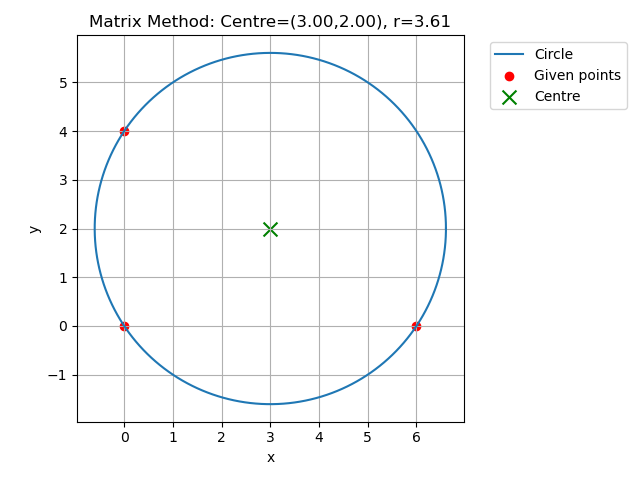
\includegraphics[width=0.9\columnwidth]{figs/newcentre.png}
    \caption{}
    \label{fig:placeholder}
\end{figure}


\end{document}
